\section{An Anatomy of Early Breast Cancers}
Breast cancer is both a common and lethal disease, having earned the dubious distinction of being both the most common and second most fatal cancer amongst females in Canada and around the world \citep{ccs2015}. Breast cancer most commonly arises in the epithelium of the mammary gland's many lactiferous ducts, which form a network that delivers to the nipple the milk that is secreted by the lobules of the mammary gland; which is another common origin of breast carcinomas (\emph{Figure \ref{anatomy}}). The epithelium of the lactiferous duct is highly organised, with well-defined tissue and cell polarity that is integral to the structure and function of the duct. The tube-like lactiferous duct is comprise of an epithelial inner-layer, which forms a hollow lumen and is surrounded by an outer layer of myoepithelial cells which express smooth-muscle actin (SMA) whose muscle-like contractile properties biomechanically deliver milk along the duct in response to hormonal signalling \citep{Hamperl_1970}.\par

\begin{figure}[ht!]
	\centering
	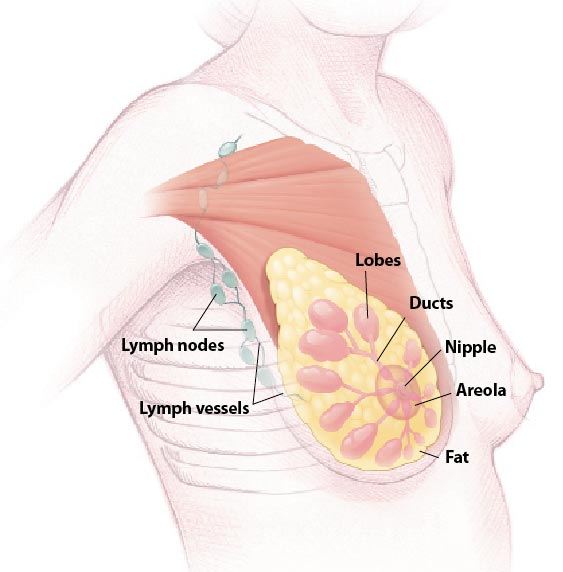
\includegraphics[width=100mm]{figures/breast_anatomy.jpg}
	\caption{Diagram of the human mammary gland and its ducts and lobules. \citep{NIH_2010} \label{anatomy}}
\end{figure}

\subsection{Stages of Early Breast Cancer Progression}
When diagnosing a suspected early breast cancer, pathologists analyse needle-core biopsies with the aim of identifying and classifying any lesions that may be present. Classification of lesions allow medical professionals to better understand the nature of the particular disease, what treatment is most appropriate, and what statistical outcomes are associated with the lesion.\par

The early stages of breast cancer manifest as pre-invasive, hyper-proliferative lesions that exhibit progressive and gradual deterioration of this epithelial organisation. These lesions belong to four histologically distinct classes: Usual Hyperplasia (UH), Flat Epithelial Atypia (FEA), Atypical Ductal Hyperplasia (ADH) (or Atypical Lobular Hyperplasia [ALH] when referring to the less common lobular lesion), and Ductal Carcinoma {\it In Situ} (DCIS).\par

Ductal or lobular hyperplasias that do not present with abnormal tissue architecture or dysplasia are classified as Usual Hyperplasia (UH), or alternatively Proliferative Disease without Atypia (PDWA). These lesions confer a relative risk of later developping breast cancer as high as 1.9, although this increase in risk is not considered sufficient to warrant any prophylactic measures, including increased follow-up \citep{mommers2001}. While UH is traditionally believed to progress serially through ADH, DCIS and ultimately IDC due to early Loss of Homozygosity (LOH) analysis, more recent cytokeratin immunophenotype and genetic hybridisation analysis has contested the evolutionary relationship between UH and other proliferative breast lesions \citep{oconnell1994, boecker2002}.\par

ADH lesions are neoplasias of the lactiferous duct that exhibit subtle dysplasia (as evidenced by nuclear hyperchromaticity), and can form micropapillary or cribiform patterns \citep{page1959,dion2016}. Of the estimated one million instances of benign breast cancer detected in the USA each  year, 10\% are classified as ADH \citep{simpson2009}. While  these lesions have been long-known and extensively proven to impart a low relative risk of malignant disease (approximately 4), recent long-term follow-up studies have shown that one in eight individuals will develop more advanced (local or invasive) breast cancers ten years after their diagnosis. This proportion increases to 46\% in individuals with more than one atypical foci twenty-five years after diagnosis \citep{hartmann2015}.\par

Arising in the terminal duct-lobule unit of the breast, FEA lesions are a purported precursor to early low-grade ductal carcinomas, and in this regard are similar to ADH. Unlike ADH however, FEA lesions are far more uncommon, never present with complex architectural patterns (thus the indication ``flat''), and are characterised by multi-layered dilated ascini often made-up of columnar cells \citep{pinder2017}. While ADH is suspected to arise from FEA lesions due their frequent coincidence, FEA is not independently associated with a long-term increased risk of breast cancer, leaving the matter unclear \citep{bombonati2011,lerwill2008,acott2016}.

%
% [ X ] poorly differentiated = >60% chance of recurrence (badve)
% [ X ] 500% increase of DCIS occurrence between 1983 to 2003 (kerlikowske)
% [   ] minor decrease in 10-year recurrence (21%-14%)
% - Surgery-Only 10yr (26%-19), Surgery+RTx (13%-11%); '78-'10 (Subhedar)
% [ X ] SMR after DCIS diagnosis is avg 1.8 (narod)
% [ X ] 30%-40% reoccur with invasive (Page, Betsill)
%


Benign early lesions go on to progress into localised malignant disease, which in the lactiferous duct is termed ductal carcinoma {\it in situ} (DCIS). DCIS is classified as a Stage 0 cancer and accounts for 20\% of all diagnosed breast cancers in the USA in 2003; representing a 500\% increase in occurrence over 20 years \citep{bleicher2013, kerlikowske2010}.\par

While DCIS has a relatively low average standardised mortality ratio (SMR) of 1.8, an estimated 30-50\% of cases reoccur as invasive breast cancers \citep{narod2015,page1982,betsill1978}. When further stratified by how well the lesion is differentiated, individuals with lesions classified as poorly differentiated (using the European Pathologists Working Group guidelines) have recurrence rates above 60\% \citep{badve1998}. At this early stage of cancer progression, the apical domain of the lumenal epithelium has begun to shrink, resulting in abnormally small lumen (a phenotype referred to as ``lumenal collapse'' herein). Our understanding of the processes by which transformed mammary duct epithelium undergoes lumenal collapse is still developing, but recent studies have described a mechanism by which lumenal tension is lost as myosin II and RhoA activity is greatly decreased at the lumenal membrane of DCIS lesions \citep{halaoui2017}. \par

The lesion becomes an invasive ductal carcinoma (IDC, or ILC in the lobular instances) when epithelial cells breach the surrounding myoepithelial layer of the duct and infiltrate into extra-cellular matrix (ECM). By this stage, cellular polarity is entirely disrupted and the apical membrane domain has completely disappeared.\par

\subsection{Intrinsic Molecular Subtypes of Cancer}

While the stage of a breast lesion may indicate its progression, even lesions of the same stage are heterogenous in their gene expression and their response to therapy. To address this heterogeneity, microarray studies of recent years have identified five ``intrinsic'' molecular subtypes through unsupervised classification of the gene expression data \citep{perou2000,prat2015}. \par

Understanding the molecular subtype is an important tool for medical practitioners, as breast cancer lesions of different subtypes are associated with different patient outcomes and respond differently to treatment \citep{engstrom2013,rouzier2005}. An alternative to microarray studies, molecular subtypes can be inferred by testing biopsy tissue for the co-occurence of a number of molecular markers, as determined by routine immunohistochemical(IHC) studies. These markers range from hormone receptors (estrogren/progesteron receptors, and human epidermal growth factor receptor 2) to proliferation markers (Ki67) (See \emph{Figure \ref{subtype_flowchart}}).

Molecular subtypes of pre-invasive DCIS lesions have been shown to be detectable in a similar fashion to their invasive counter-parts, although relative frequencies between the two being significantly different \citep{tamimi2008,clark2011}. Notably, triple-negative and basal-like phenotypes are occur very rarely in DCIS when compared to invasive disease.

\begin{figure}[ht!]
	\centering
	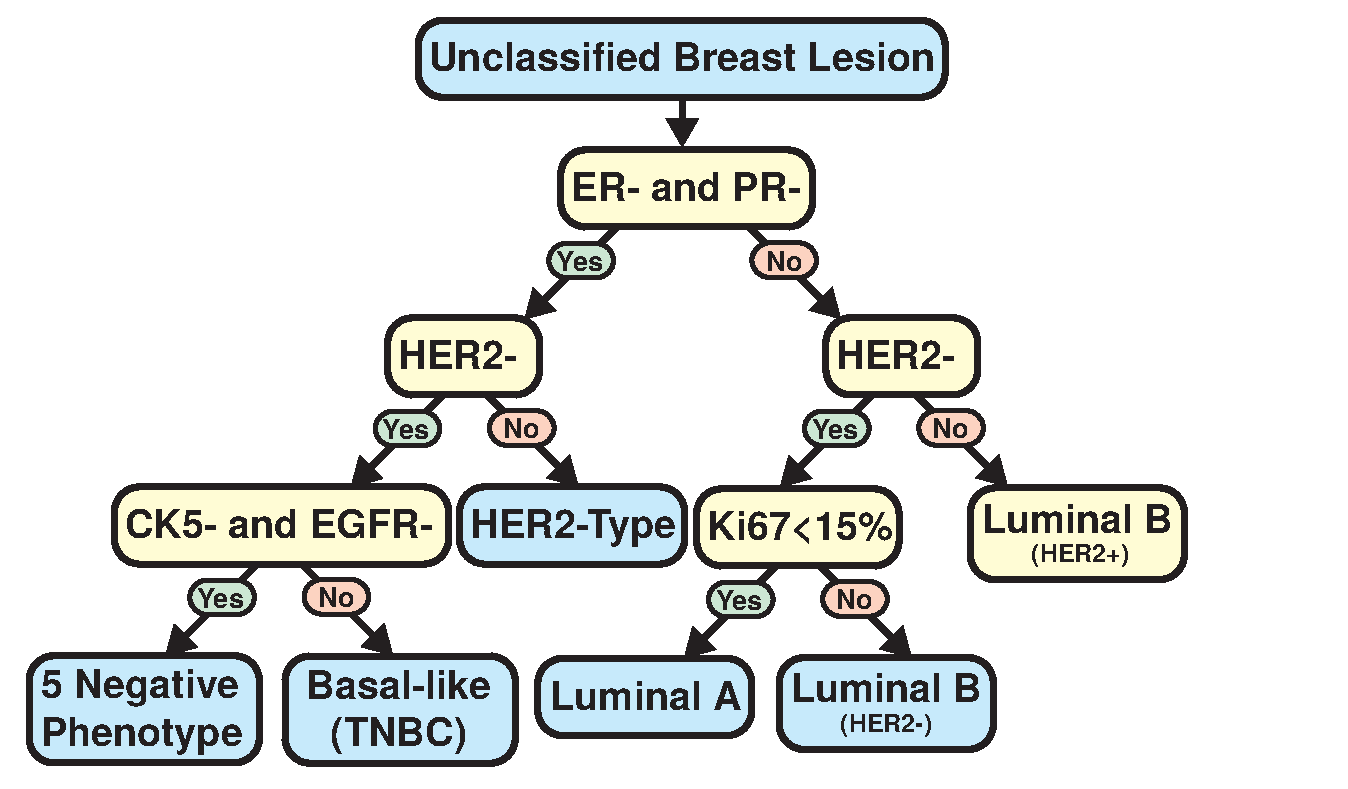
\includegraphics[width=150mm]{figures/subtype_flowchart.pdf}
	\caption{Flowchart for the determination of the molecular subtype of breast lesions. Molecular subtype can be determined by staining for the estrogen, progesteron, epithelial growth factor receptors, and human epidermal growth factor receptor 2 (ER, PR, EGFR, and HER2, respectively), as well as the basal/myoepithelial marker cytokeratin 5 (CK5) and proliferation marker Ki67. Adapted from \cite{engstrom2013}. \label{subtype_flowchart}}
\end{figure}